%! Author = Carlos Delgado
%! Author = Emilio Mena
%! Date = 20-mar-2020

\documentclass{article}
\usepackage[utf8]{inputenc}

\title{MC PROTECT}
\author{Carlos}
\author{Emilio}
\date{March 2020}

\usepackage{natbib}
\usepackage{graphicx}

\begin{document}

\maketitle

\section{Introduction}
Aqui va la intro

%! esto es una figura (imagen)
\begin{figure}[h!]
\centering
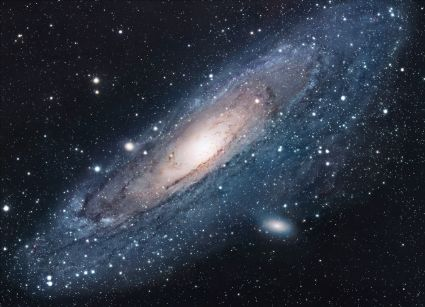
\includegraphics[scale=1.7]{universe}
\caption{The Universe}
\label{fig:universe}
\end{figure}
%! aquí acaba la figura

%! otra seccion
\section{Conclusion}
%! esto es una cita el ~\citep{XX} marca que hace referencia al texto XX
``I always thought something was fundamentally wrong with the universe''~\citep{adams1995hitchhiker}


%! así se agrega la bibliografía
\bibliographystyle{plain}
\bibliography{references}
\end{document}
